\documentclass{article}
\usepackage[english]{babel}
\usepackage[utf8]{inputenc}
\usepackage{fancyhdr}
\usepackage{amsmath}
\usepackage{pdfpages}
\usepackage{graphicx}
\graphicspath{ {./image/} }
\pagestyle{fancy}
\fancyhf{}
\rhead{CS760}
\lhead{Cheng-Wei Lu}
\rfoot{Page \thepage}

\begin{document}

\section*{CS 760 Homework 5 by Cheng-Wei Lu}

\subsection*{Problem 5.1}
\subsubsection*{(a)}
	For this problem, I created a KNN model that takes in the training data at the time when it is created. Then, I created  a predict method for my KNN class, where the distances between the given test features and training data will be calculated. Then the model will choose the top K nearest data and use their y values as equal votes to determine the prediction value. The code is in the appendix following the title, "KNN Model".
\subsubsection*{(b)}
	I first converted all features into binary features. This is because it is harder for us to convert binary features to continuous features, and I think each feature should be treated equally. Therefore, I converted all of them into binary features. For each non-binary feature, I use its average as a standard to decide the binary transformation of each data. I use average because in reality, we often divide data in two parts with average. Therefore, I think it would also be reasonable if I use average here. If the original feature is greater than the average, it will be converted to 1. If not, it will be converted to 0. The average for passenger class is 2.3, age is 29.4, siblings/spouses aboard is 0.5, parents/children aboard is 0.4 and fare is 32.3. 
\subsubsection*{(c)}
	According to the conversion rule, my data input to the KNN model will be,
	\begin{equation*}	
	\begin{pmatrix} 1 \text{(class)}\\ 0 \text{(sex)}\\ 0\text{(age)}\\ 0\text{(siblings/spouses aboard)}\\0\text{(parents/children aboard)}\\ 1\text{(fare)}\end{pmatrix} 
	\end{equation*}.
	
	According to my model , I wouldn't have survived. The graph shows that my probability of survival will never exceed 0.5.\\
	
	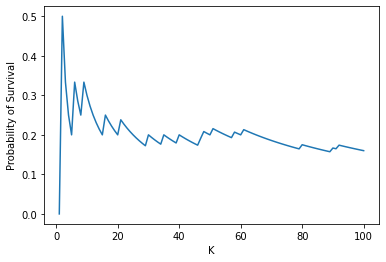
\includegraphics[scale=0.5]{1_c}
	
\subsubsection*{(d)}
	I think the best choice of K will be 3 or 4, because when K is larger than that, the probability will start to converge .
	
\subsubsection*{(e)}
	My way to look at the confidence for my prediction is to use 10-cross validation to evaluate the validation accuracy. In this model, it is 0.7881. That means about 78.81\% chance that my prediction will be right.



\subsection*{Problem 5.2}
\subsubsection*{(a)}
	The code is in the appendix following the title, "Naive Bayes Model".	I use original data instead of converting them into binary features in this problem.
\subsubsection*{(b)}
	For passenger class, I model it with multinomial distribution, since there are three classes in the feature, and $\frac{\text{class 1} + \text{class 3}}{2} \neq \text{class 2}$ . I model gender with binomial distribution. I model all remaining features with Gaussian distribution, since none of them is nominal data.
\subsubsection*{(c)}
	My data input to the Naive Bayes model will be,

	\begin{equation*}	
	\begin{pmatrix} 2 \text{(class)}\\ 0 \text{(sex)}\\ 25\text{(age)}\\ 0\text{(siblings/spouses aboard)}\\0\text{(parents/children aboard)}\\ 53.1\text{(fare)}\end{pmatrix} 
	\end{equation*}.
	According to my model, my posterior probability to die is $2.46\times10^{-6}$, which is bigger than the probability that I will survive $9.85\times 10^{-7}$. Therefore, I will die.
	
\subsubsection*{(d)}
	My way to look at the confidence for my prediction is to use 10-cross validation to evaluate the validation accuracy. In this model, it is 0.7780. That means about 77.8\% chance that my prediction will be right.

\subsection*{Problem 5.3}
	I would like to use logistic regression more, because with logistic regression, we analyze more detailedly on the relationship between the coefficient of a feature with the prediction result. In KNN, we are not able to get the relationship of features, and in Naive Bayes, we assume the independence between two features, while I think it is more reasonable for us to consider the relationship among them.
	
	
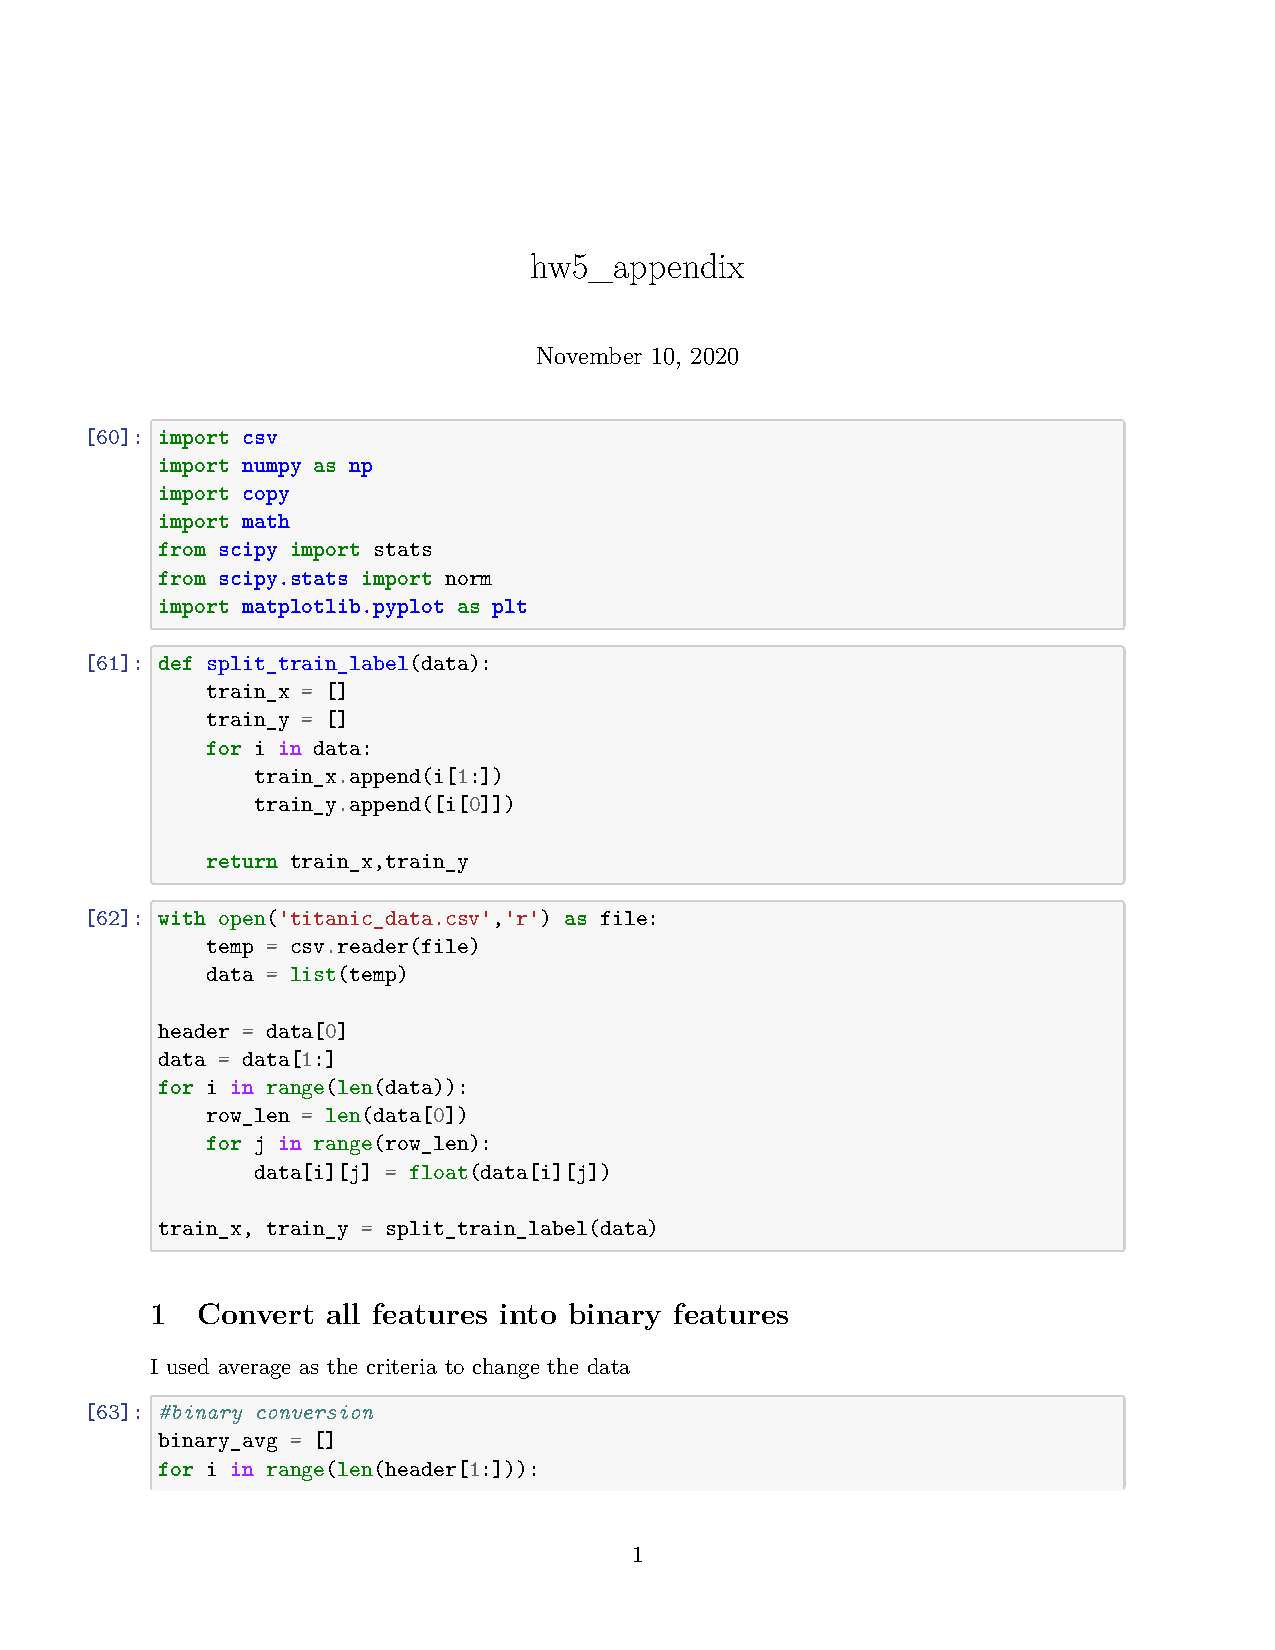
\includepdf[page={1-}]{hw5_appendix}


\end{document}